\begin{flushright} {\tiny {\color{gray} (tikz\_staggered2D\_u2.tex)}} \end{flushright}
%~~~~~~~~~~~~~~~~~~~~~~~~~~~~~~~~~~~~~~~~~~~~~~~~~~~~~~~~~~~~~~~~~~~~~~~~~~~~~~~~~~~~~~~~~~~~~~~~~~

\begin{center}
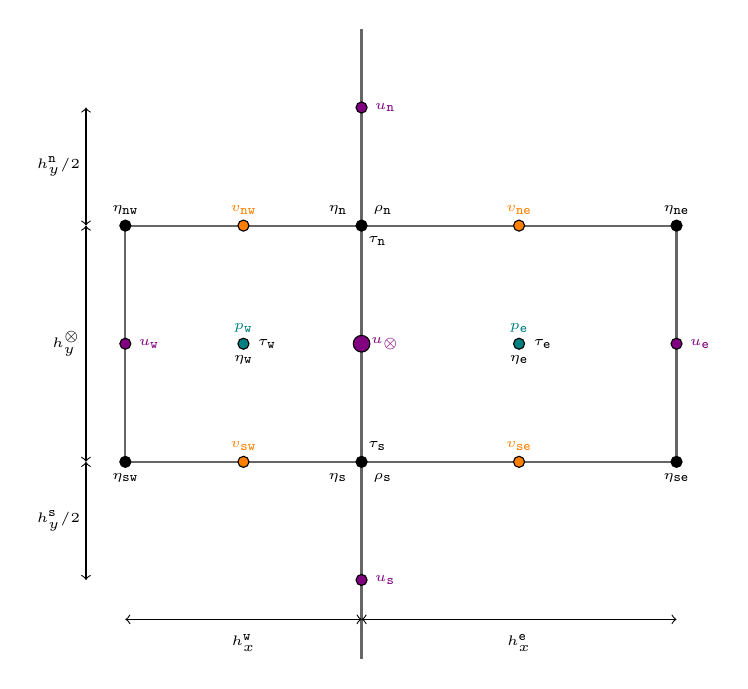
\begin{tikzpicture}
%\draw[fill=gray!23,gray!23](0,0) rectangle (10,9);
%\draw[step=0.5cm,gray,very thin] (0,0) grid (10,9); %background grid

\draw[thick,black!60] (1,3) -- (8,3) -- (8,6) -- (1,6) -- cycle ; 
\draw[thick,black!60] (4,0.5) -- (4,8.5)  ;   

%---------------------------------------------------
%horizontal arrows
\draw[<->,black] (1,1) -- (4,1) ; \node[] at (2.5,0.7) {\tiny $h_x^{\tt w}$};
\draw[<->,black] (4,1) -- (8,1) ; \node[] at (6,0.7) {\tiny $h_x^{\tt e}$};

%vertical arrows
\draw[<->,black] (0.5,1.5) -- (0.5,3) ; \node[] at (0.15,2.25) {\tiny $h_y^{\tt s}/2$};  
\draw[<->,black] (0.5,3) -- (0.5,6)   ; \node[] at (0.25,4.5) {\tiny $h_y^{\otimes}$};
\draw[<->,black] (0.5,6) -- (0.5,7.5) ; \node[] at (0.15,6.75) {\tiny $h_y^{\tt n}/2$};  

%---------------------------------------------------
\node[] at (2.5,6.2) {\tiny \color{orange} $v_{\tt nw}$};
\node[] at (2.5,3.2) {\tiny \color{orange} $v_{\tt sw}$};
\node[] at (6,6.2) {\tiny \color{orange} $v_{\tt ne}$};
\node[] at (6,3.2) {\tiny \color{orange} $v_{\tt se}$};
\draw[black,fill=orange] (2.5,6)   circle (2pt);
\draw[black,fill=orange] (2.5,3)   circle (2pt);
\draw[black,fill=orange] (6,6)   circle (2pt);
\draw[black,fill=orange] (6,3)   circle (2pt);

%--------------------------------------------------
\draw[black,fill=violet] (4,1.5)   circle (2pt);
\draw[black,fill=violet] (4,4.5)   circle (3pt);
\draw[black,fill=violet] (4,7.5)   circle (2pt);
\draw[black,fill=violet] (1,4.5)   circle (2pt);
\draw[black,fill=violet] (8,4.5)   circle (2pt);
\node[] at (4.3,1.5) {\tiny \color{violet} $u_{\tt s}$};
\node[] at (4.3,4.5) {\tiny \color{violet} $u_\otimes$};
\node[] at (4.3,7.5) {\tiny \color{violet} $u_{\tt n}$};
\node[] at (1.3,4.5) {\tiny \color{violet} $u_{\tt w}$};
\node[] at (8.3,4.5) {\tiny \color{violet} $u_{\tt e}$};

\draw[black,fill=black] (1,3)   circle (2pt); 
\draw[black,fill=black] (4,3)   circle (2pt); 
\draw[black,fill=black] (8,3)   circle (2pt); 
\draw[black,fill=black] (1,6)   circle (2pt); 
\draw[black,fill=black] (4,6)   circle (2pt); 
\draw[black,fill=black] (8,6)   circle (2pt); 

%------------------------------------------------
\draw[black,fill=teal] (2.5,4.5)   circle (2pt);
\draw[black,fill=teal] (6,4.5)   circle (2pt);
\node[] at (2.5,4.7) {\tiny \color{teal} $p_{\tt w}$};
\node[] at (6,4.7) {\tiny \color{teal} $p_{\tt e}$};

\node[] at (4.27,2.8) {\tiny $\rho_{\tt s}$};
\node[] at (4.27,6.2) {\tiny $\rho_{\tt n}$};
\node[] at (2.5,4.3) {\tiny $\eta_{\tt w}$};
\node[] at (6,4.3) {\tiny $\eta_{\tt e}$};
\node[] at (3.7,2.8) {\tiny $\eta_{\tt s}$};
\node[] at (3.7,6.2) {\tiny $\eta_{\tt n}$};
\node[] at (8,6.2) {\tiny $\eta_{\tt ne}$};
\node[] at (1,6.2) {\tiny $\eta_{\tt nw}$};
\node[] at (8,2.8) {\tiny $\eta_{\tt se}$};
\node[] at (1,2.8) {\tiny $\eta_{\tt sw}$};

\node[] at (6.3,4.5) {\tiny $\tau_{\tt e}$};
\node[] at (2.8,4.5) {\tiny $\tau_{\tt w}$};

\node[] at (4.2,3.2) {\tiny $\tau_{\tt s}$};
\node[] at (4.2,5.8) {\tiny $\tau_{\tt n}$};

\end{tikzpicture}
\end{center}










